\subsubsection{Financial Data Structures}

\begin{figure}[H]
\centering
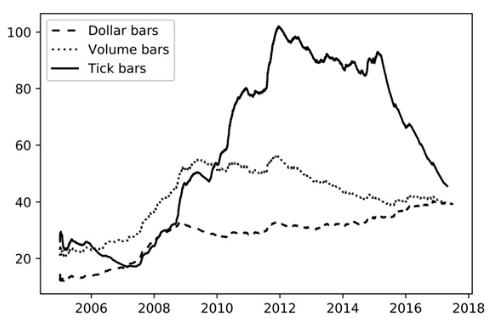
\includegraphics[scale=0.55]{figures/intro/standardbars}
\caption{Average daily frequency of tick, volume, and dollar bars}
\end{figure}

\begin{remark} \hlt{Standard BARS}\\
For converting a stream of irregularly timed observations into a homogeneous series through regular sampling.
\begin{enumerate}[label=\roman*.]
\setlength{\itemsep}{0pt}
\item \textbf{Time Bars:} Sample data at fixed time intervals. Typically record information such as the timestamp, volume-weighted average price (VWAP), open price, close price, high price, low price, and volume.\\
As markets do not operate in constant time intervals, time bars tend to oversample during periods of low activity and undersample during high-activity periods. Consequently, they often exhibit undesirable statistical properties such as serial correlation, heteroscedasticity, and non-normal return distributions.
\item \textbf{Tick Bars:} Created by sampling each time a specified number of transactions occur, thereby aligning the sampling process with the arrival of market information.\\
This method often results in returns that are closer to IID normal (\cite{Thierry_Helyette_2000}). Nonetheless, care must be taken to address outliers since many exchanges conduct opening and closing auctions where the order book may accumulate unmatched bids and offers. Additionally, order fragmentation can introduce some arbitrariness in the tick count.
\item \textbf{Volume Bars:} Generated by sampling whenever a predetermined number of security units are traded.\\
Volume bars generally yield better statistical properties than tick bars and serve as a useful tool for studying market microstructure theories.
\item \textbf{Dollar Bars:} Formed by sampling each time a fixed monetary value is exchanged. This approach is particularly useful for analyses involving significant price fluctuations and is robust to corporate actions (e.g., splits, reverse splits, new share issuances, or share buybacks).\\
Moreover, the bar size can be adjusted dynamically based on factors such as a company’s free-floating market capitalization or the total amount of issued debt.
\end{enumerate}
\end{remark}

\begin{remark} \hlt{Information-Driven Bars}\\
Sample more frequently when new (micro-structural) information enters the market.
\begin{enumerate}[label=\roman*.]
\setlength{\itemsep}{0pt}
\item \textbf{Tick Imbalance Bars:} Formed whenever the cumulative tick imbalance exceeds its expected threshold.\\
Consider a sequence of ticks $\{(p_t, v_t)\}_{t=1}^{T}$, where $p_t$ and $v_t$ denote the price and volume of tick $t$, respectively. A tick rule defines the sequence $\{b_t\}_{t=1}^{T}$ by
\begin{align}
b_t =
\begin{cases}
b_{t-1}, & \text{if } \Delta p_t = 0, \\
\frac{\lvert \Delta p_t \rvert}{\Delta p_t}, & \text{if } \Delta p_t \neq 0.
\end{cases} \nonumber
\end{align}
The tick imbalance at time $T$ is then given by
\[ \theta_T = \sum_{t=1}^{T} b_t. \]
Its expected value at the beginning of a bar is computed as
\[ E_0[\theta_T] = E_0[T]\big(P[b_t = 1] - P[b_t = -1]\big) = E_0[T]\big(2P[b_t = 1] - 1\big), \]
where $E_0[T]$ is the expected tick bar size, and $P[b_t = 1]$ and $P[b_t = -1]$ are the unconditional probabilities of a tick being classified as a buy or a sell, respectively. In practice, $E_0[T]$ and $(2P[b_t = 1] - 1)$ are estimated using an exponentially weighted moving average from previous bars.\\
Define the Tick Imbalance Bar (TIB) as the smallest contiguous subset of ticks such that
\[ T^{*} = \arg \min_T \{ \lvert \theta_T \rvert \geq E_0[T] \, \vert \, 2P[b_t = 1] - 1 \}. \]
When the observed imbalance $\theta_T$ exceeds the expected value, a lower $T$ will satisfy the condition.

\item \textbf{Volume/Dollar Imbalance Bars:} These bars are triggered when the imbalance in volume or dollar amount deviates from its expectation. First, define the imbalance at time $T$ as
\[ \theta_T = \sum_{t=1}^{T} b_t v_t, \]
where $v_t$ represents either the number of units traded (for Volume Imbalance Bars, VIB) or the dollar amount exchanged (for Dollar Imbalance Bars, DIB). The expected imbalance is calculated as
\begin{align}
E_0[\theta_T] &= E_0\Bigg[\sum_{t: b_t=1}^{T} v_t\Bigg] - E_0\Bigg[\sum_{t: b_t=-1}^{T} v_t\Bigg] \nonumber \\
&= E_0[T]\Big(P[b_t = 1]E_0[v_t \vert b_t = 1] - P[b_t = -1]E_0[v_t \vert b_t = -1]\Big) \nonumber \\
&= E_0[T]\Big(v^+ - v^-\Big) \nonumber
\end{align}
or equivalently,
\[ E_0[\theta_T] = E_0[T]\Big(2v^+ - E_0[v_t]\Big). \]
In practice, $E_0[T]$ and $(2v^+ - E_0[v_t])$ are estimated as an exponentially weighted moving average from previous bars. Next, define the VIB or DIB as the smallest contiguous subset of ticks satisfying
\[ T^* = \arg \min_T \{ \lvert \theta_T \rvert \geq E_0[T] \, \vert \, 2v^+ - E_0[v_t] \}. \]
Thus, when the observed imbalance exceeds the expected value, the bar is triggered.

\item \textbf{Tick Runs Bars:} These bars are formed when the sequence of consecutive buys or sells (i.e., runs) deviates from expectation. This is particularly relevant when large traders sweep the order book, use iceberg orders, or split parent orders into multiple child orders, leaving a trace in the sequence $\{b_t\}_{t=1}^{T}$.\\
Define the run length as
\[ \theta_T = \max \left\{ \sum_{t: b_t = 1}^{T} b_t - \sum_{t: b_t = -1}^{T} b_t \right\}. \]
The expected run length at the start of the bar is given by
\[ E_0[\theta_T] = E_0[T] \max\{P[b_t = 1], 1 - P[b_t = 1]\}. \]
In practice, $E_0[T]$ and $P[b_t = 1]$ are estimated via an exponentially weighted moving average from prior bars. The Tick Runs Bar (TRB) is then defined as the smallest contiguous subset of ticks such that
\[ T^* = \arg \min_T \Big\{ \theta_T \geq E_0[T] \max\{P[b_t = 1], 1 - P[b_t = 1]\} \Big\}. \]
This definition implies that when $\theta_T$ exceeds the expected run length, a bar is formed. (Note: alternatively, one may count the number of ticks on each side without netting them off.)

\item \textbf{Volume/Dollar Runs Bars:} These bars are triggered when the cumulative volume or dollar amount traded by one side exceeds its expected value.\\
First, define the run imbalance as
\[ \theta_T = \max \left\{ \sum_{t: b_t = 1}^{T} b_t v_t - \sum_{t: b_t = -1}^{T} b_t v_t \right\}, \]
where $v_t$ is traded volume (for Volume Runs Bars, VRB) or dollar amount (for Dollar Runs Bars, DRB).\\
The expected imbalance is then computed as
\begin{align}
E_0[\theta_T] = E_0[T] \max \Big\{ P[b_t = 1]E_0[v_t \vert b_t = 1],\ & (1 - P[b_t = 1])E_0[v_t \vert b_t = -1] \Big\}. \nonumber
\end{align}
In practice, $E_0[T]$, $P[b_t = 1]$, $E_0[v_t \vert b_t = 1]$, and $E_0[v_t \vert b_t = -1]$ are estimated using exponentially weighted moving averages from prior bars. Define VRB or DRB as the smallest contiguous subset of ticks satisfying
\[ T^* = \arg \min_T \Big\{ \theta_T \geq E_0[T] \max \Big\{ P[b_t = 1]E_0[v_t \vert b_t = 1],\ (1 - P[b_t = 1])E_0[v_t \vert b_t = -1] \Big\} \Big\}. \]
Thus, when the observed run imbalance exceeds the expected value, a bar is triggered.
\end{enumerate}
\end{remark}

\begin{definition} \hlt{Multi-Product Series: ETF Trick}\\
A technique to model a basket of securities as if it were a single cash product, effectively transforming a complex multi-product dataset into a unified series that mimics a total return ETF.
\end{definition}

\begin{method} \hlt{ETF Trick}\\
The following steps produce a time series that reflects the value of a \$1 investment, with changes in the series representing profit and loss (PnL). The series remains strictly positive and incorporates implementation shortfall. The bars include:
\begin{enumerate}[label=\roman*.]
\setlength{\itemsep}{0pt}
\item The raw open price for each instrument $i = 1, \ldots, I$ at bar $t$, denoted by $o_{i,t}$.
\item The raw close price for each instrument $i = 1, \ldots, I$ at bar $t$, denoted by $p_{i,t}$.
\item The USD value of one point of instrument $i = 1, \ldots, I$ at bar $t$, denoted by $\varphi_{i,t}$ (includes forex rate).
\item The trading volume for instrument $i = 1, \ldots, I$ at bar $t$, denoted by $v_{i,t}$.
\item Any carry, dividend, or coupon paid by instrument $i$ at bar $t$, denoted by $d_{i,t}$ (this variable can also account for margin or funding costs).
\end{enumerate}
All instruments $i = 1, \ldots, I$ must be tradable at each bar $t = 1, \ldots, T$. Even if some instruments are not continuously tradable throughout the interval $[t-1, t]$, they should be tradable at both times $t-1$ and $t$.\\
For a basket of securities with an allocation vector $\omega_t$ that is rebalanced (or rolled) on a set of bars $B \subseteq \{1, \ldots, T \}$, the \$1 investment value series $\{K_t\}$ is derived as follows:
\begin{align}
h_{i,t} &= 
\begin{cases}
\displaystyle \frac{\omega_{i,t} K_t}{o_{i, t+1} \varphi_{i,t} \sum_{i=1}^I \lvert \omega_{i,t} \rvert} , & \text{if } t \in B, \\[1ex]
h_{i, t-1}, & \text{otherwise,}
\end{cases} \nonumber \\
\delta_{i,t} &=
\begin{cases}
p_{i,t} - o_{i,t}, & \text{if } (t-1) \in B, \\
\Delta p_{i,t}, & \text{otherwise,}
\end{cases} \nonumber \\
K_t &= K_{t-1} + \sum_{i=1}^I h_{i, t-1} \varphi_{i,t} (\delta_{i,t} + d_{i,t}) \nonumber
\end{align}
with the initial asset under management (AUM) set as $K_0 = 1$. Here, $h_{i,t}$ denotes the holdings of instrument $i$ at time $t$, and $\delta_{i,t}$ represents the change in market value for instrument $i$ between $t-1$ and $t$. Profits or losses are reinvested on rebalancing days (i.e., when $t \in B$), thereby avoiding negative prices. Dividends $d_{i,t}$ are already incorporated within $K_t$.\\
The normalization factor $\omega_{i,t}\left(\sum_{i=1}^I \lvert \omega_{i,t} \rvert \right)^{-1}$ is used to de-lever the allocations.\\
Let $\tau_i$ be transaction cost associated with trading $\$1$ of the instrument. Three additional variables that the strategy needs to know for every observed bar $t$ are:
\begin{enumerate}[label=\roman*.]
\setlength{\itemsep}{0pt}
\item Rebalance Costs: variable cost $\{c_t\}$ associated with allocation rebalance is
\begin{equation}
c_t = \sum\limits_{i=1}^I (\abs{h_{i, t-1}}p_{i,t} + \abs{h_{i,t}} o_{i, t+1}) \varphi_{i,t} \tau_{i} \ \ \ \forall t \in B \nonumber
\end{equation}
Note $c_t$ is not embedded in $K_t$, as shorting will generate fictitious proceeds when allocation is rebalanced.\\
In code, $\{c_t\}$ is treated as a (negative) dividend.
\item Bid-Ask Spread: the cost $\{ \tilde{c}_t \}$ of buying or selling one unit of this ETF,
\begin{equation}
\tilde{c}_t = \sum\limits_{i=1}^I \abs{h_{i, t-1}}p_{i, t} \varphi_{i,t} \tau_i \nonumber
\end{equation}
When a unit is bought or sold, strategy must charge this cost $\tilde{c}_t$.
\item Volume: volume traded $\{v_t \}$ is determined by least active member in the basket. Let $v_{i,t}$ be volume traded by instrument $i$ over bar $t$. The number of tradable basket units is
\begin{equation}
v_t = \min_i \left\{ \frac{v_{i,t}}{\abs{h_{i, t-1}}} \right\} \nonumber
\end{equation}
\end{enumerate}
Transaction costs functions may not be linear, and can be simulated by the strategy.
\end{method}

\begin{method} \hlt{ETF Trick: Computation of Allocation Vector with PCA}\\
Consider an IID multivariate Gaussian process characterized by a mean vector $\mu$ (of size $N \times 1$) and a covariance matrix $V$ (of size $N \times N$). First, perform the spectral decomposition
\[ VW = W \Lambda, \]
with the columns of $W$ rearranged so that the diagonal entries of $\Lambda$ are in descending order. Given an allocation vector $\omega$, the portfolio risk is
\[ \sigma^2 = \omega' V \omega = \omega' W \Lambda W' \omega = \beta' \Lambda \beta = (\Lambda^{1/2} \beta)'(\Lambda^{1/2} \beta)', \]
where $\beta$ represents the projection of $\omega$ onto the orthogonal basis defined by $W$. Since $\Lambda$ is diagonal, we have
\[ \sigma^2 = \sum_{n=1}^N \beta_n^2 \Lambda_{n,n}. \]
The risk contribution from the $n$th component is then
\[ R_n = \frac{\beta_n^2 \Lambda_{n,n}}{\sigma^2} = \frac{[W' n]^2_n \Lambda_{n,n}}{\sigma^2}, \]
with the property that $\sum_{n=1}^N R_n = 1$, where $1_N$ is an $N$-dimensional vector of ones.\\
To compute an allocation vector $\omega$ that satisfies a user-defined risk distribution $R$, note that
\[ \beta = \left\{ \sigma \sqrt{\frac{R_n}{\Lambda_{n,n}}} \right\}_{n = 1}^{N}, \]
which represents the allocations in the new orthogonal basis. Allocation in original basis is then recovered by
\[ \omega = W \beta. \]
Rescaling $\omega$ proportionally adjusts $\sigma$, thus preserving the risk distribution.
\end{method}

\begin{method} \hlt{ETF Trick: Single Futures Roll}\\
To generate a non-negative, continuously rolled series for a \$1 investment, proceed as follows:
\begin{enumerate}[label=\roman*.]
\setlength{\itemsep}{0pt}
\item Compute the time series of rolled futures prices.
\item Calculate the return $r$ as the percentage change of the rolled price relative to the previous roll price.
\item Construct the price series using these returns.
\end{enumerate}
\end{method}

The methods described above enable the production of a continuous, homogeneous, and structured dataset from a collection of unstructured financial data. It is important to note, however, that many machine learning algorithms do not scale well with extremely large sample sizes; their accuracy typically improves when they are trained on the most relevant examples.

\begin{method} \hlt{Sampling for Reduction}\\
To reduce volume of data used for fitting a machine learning algorithm, downsampling techniques can be applied:
\begin{enumerate}[label=\roman*.]
\setlength{\itemsep}{0pt}
\item \textbf{Sequential Sampling:} Sample the data at a constant step size (i.e., using linspace sampling).
\item \textbf{Random Sampling:} Select data points randomly according to a uniform distribution.
\end{enumerate}
Note that neither sampling method guarantees that the most relevant observations are retained.
\end{method}

\begin{method} \hlt{Event-Based Sampling: CUMSUM Filter} \\
In many cases, decisions (or bets) are made after a significant event. To enable a machine learning algorithm to learn a predictive function in such scenarios, the CUSUM filter can be employed. The CUSUM filter is a quality-control method designed to detect shifts in the mean value of a measured variable away from a target.\\
Let $\{y_t\}_{t=1}^{T}$ be IID observations from a locally stationary process. The cumulative sum is defined recursively by
\[ S_t = \max\{0,\, S_{t-1} + y_t - E_{t-1}[y_t]\}, \quad S_0 = 0. \]
An action will be recommended at the first $t$ satisfying $S_t \geq h$ for some threshold $h$ (filter size).\\
Note $S_t = 0$ whenever $y_t = E_{t-1}[y_t] - S_{t-1}$, The zero floor means some downward deviations will be skipped.\\
The filter is set up to identify a sequence of upside divergences from any reset level zero.\\
The threshold is activated when
\begin{equation}
S_t \geq h \Leftrightarrow \exists \tau \in [1, t] \ \vert \ \sum\limits_{i=\tau}^t (y_i - E_{i-1}[y_t]) \geq h \nonumber
\end{equation}
The concept can be extended to capture symmetric movements by defining
\begin{align}
S^+_t &= \max\{0,\, S^+_{t-1} + y_t - E_{t-1}[y_t]\}, \quad S^+_0 = 0, \nonumber \\
S^-_t &= \min\{0,\, S^-_{t-1} + y_t - E_{t-1}[y_t]\}, \quad S^-_0 = 0, \nonumber \\
S_t   &= \max\{S^+_t,\ -S^-_t\}. \nonumber
\end{align}
\end{method}